% Note that the text in the [] brackets is the one that will
% appear in the table of contents, whilst the text in the {}
% brackets will appear in the main thesis.

%% CHAPTER HEADER /////////////////////////////////////////////////////////////////////////////////////
\chapter[Results and Discussions]{Results and Discussions}
\label{ch5}

%% CHAPTER INTRODUCTION ///////////////////////////////////////////////////////////////////////////////
The results and discussion regarding delamination identification in CFRP plates will be presented. 
Accordingly, to verify the developed DL models, we evaluated them on unseen numerical test cases and further on experimental test cases.
In the first section, we will present and discuss the results of the developed CNN classifier. 
In the second section, we will present and discuss the results of the five developed FCN models, and accordingly, a comparison between them will be made.
In the third section, the results, and discussion regarding the developed AE-ConvLSTM model are presented.
In section four, the results of applying a super-resolution image reconstruction of full wavefield will be presented. 

%% INCLUDE SECTIONS ///////////////////////////////////////////////////////////////////////////////////

%% SECTION HEADER /////////////////////////////////////////////////////////////////////////////////////
\section{CNN classifier models}
\label{sec51}

In this section, the predicted outputs of utilising the CNN classifier on the selected four RMS numerical cases (from the top of the plate), which have delaminations of different locations, shapes, and angles.

In the first numerical case, the delamination is located at left edge of the plate, as shown in Fig.~\ref{fig:GT_case_448}, representing its ground truth (GT).
The predicted output using (\(14\times14\)) and (\(16\times16\)) patches are presented in Fig.~\ref{fig:pred_7_7_case_448} and Fig.~\ref{fig:pred_8_8_case_448}.
%%%%%%%%%%%%%%%%%%%%%%%%%%%%%%%%%%%%%%%%%%%%%%%%%%%%%%%%%%%%%%%%%%%%%%%%%%%%%%%%
For second numerical case, the delamination is located at upper left corner of the plate, as shown in Fig.~\ref{fig:GT_case_456}, representing its ground truth (GT).
The predicted output using (\(14\times14\)) and (\(16\times16\)) patches are presented in Fig.~\ref{fig:pred_7_7_case_456} and Fig.~\ref{fig:pred_8_8_case_456}.
%%%%%%%%%%%%%%%%%%%%%%%%%%%%%%%%%%%%%%%%%%%%%%%%%%%%%%%%%%%%%%%%%%%%%%%%%%%%%%%%
In third numerical case, the delamination is located near to center upper edge of the plate, as shown in Fig.~\ref{fig:GT_case_438}, representing its ground truth (GT).
The predicted output using (\(14\times14\)) and (\(16\times16\)) patches are presented in Fig.~\ref{fig:pred_7_7_case_438} and Fig.~\ref{fig:pred_8_8_case_438}.
%%%%%%%%%%%%%%%%%%%%%%%%%%%%%%%%%%%%%%%%%%%%%%%%%%%%%%%%%%%%%%%%%%%%%%%%%%%%%%%%
It is important to notice that the first, second and the third cases are considered difficult due to the edge wave reflections that have the similar patterns as delamination reflection.
However, the CNN classifiers were able to detect the delamination in such difficult cases.
%%%%%%%%%%%%%%%%%%%%%%%%%%%%%%%%%%%%%%%%%%%%%%%%%%%%%%%%%%%%%%%%%%%%%%%%%%%%%%%%
For four numerical case, the delamination is located in the upper left quarter of the plate, as shown in Fig.~\ref{fig:GT_case_397}, representing its ground truth (GT).
The predicted output using (\(14\times14\)) and (\(16\times16\)) patches are presented in Fig.~\ref{fig:pred_7_7_case_397} and Fig.~\ref{fig:pred_8_8_case_397}.
%%%%%%%%%%%%%%%%%%%%%%%%%%%%%%%%%%%%%%%%%%%%%%%%%%%%%%%%%%%%%%%%%%%%%%%%%%%%%%%%

Table~\ref{tab:table_all_numerical_cases_bounding_boxes} presents the \(IoU\) values for CNN classier with respect to the input patch size for the numerical cases shown in Fig.~\ref{fig:bounding_boxes_predictions}.
Furthermore, the mean \(IoU\) for all \(95\) test cases is \((0.16)\) and \((0.2)\) for (\(14\times14\)) and (\(16\times16\)) patches, receptively.
Consequently, it can be concluded that when increasing the input resolution (i.e., using \((16\times16)\) patches), the obtained \(IoU\) values increased.
It should also be mentioned, that for both input patches, the CNN classifier was able to detect all the delaminations for the \(95\) test cases.

Moreover, the CNN classier model was tested on experimental data, however, due to the poor quality of the obtained results, I did not present them.

%%%%%%%%%%%%%%%%%%%%%%%%%%%%%%%%%%%%%%%%%%%%%%%%%%%%%%%%%%%%%%%%%%%%%%%%%%%%%%%%
\begin{table}[ht!]
	\centering
	\caption{IoU values of numerical cases}
	\label{tab:table_all_numerical_cases_bounding_boxes}
	{
		\begin{tabular}{lcc}
			\toprule[1.5pt]
			Case & \multicolumn{2}{c}{Patches} \\ 
			\cmidrule(lr){2-3} & \multicolumn{1}{c}{\((14\times14)\)} & \multicolumn{1}{c}{\((16\times16)\)} \\			
			\midrule 
			1 & \(0.26\) & \(0.34\) \\
			2 & \(0.18\) & \(0.23\) \\
			2 & \(0.07\) & \(0.04\) \\
			4 & \(0.12\) & \(0.24\) \\
			\bottomrule[1.5pt]
		\end{tabular}
	}
\end{table}
%%%%%%%%%%%%%%%%%%%%%%%%%%%%%%%%%%%%%%%%%%%%%%%%%%%%%%%%%%%%%%%%%%%%%%%%%%%%%%%%
\begin{figure} [h!]
	\centering
	%%%%%%%%%%%%%%%%%%%%%%%%%%%%%%%%%%%%%%%%%%%%%%%%%%%%%%%%%%%%%%%%%%%%%%%%%%%%
	%%%%% case 448
	%%%%%%%%%%%%%%%%%%%%%%%%%%%%%%%%%%%%%%%%%%%%%%%%%%%%%%%%%%%%%%%%%%%%%%%%%%%%
	\begin{subfigure}[b]{0.32\textwidth}
		\centering
		\includegraphics[width=1\textwidth]{Figures/Chapter_5/m1_rand_single_delam_448.png}
		\caption{}
		\label{fig:GT_case_448}
	\end{subfigure}	
	\hfill
	\begin{subfigure}[b]{0.32\textwidth}
		\centering
		\includegraphics[width=1\textwidth]{Figures/Chapter_5/predicted_output_7_7_448.png}
		\caption{\(IoU=0.26\)}
		\label{fig:pred_7_7_case_448}
	\end{subfigure}
	\hfill
	\begin{subfigure}[b]{0.32\textwidth}
		\centering
		\includegraphics[width=1\textwidth]{Figures/Chapter_5/predicted_output_8_8_448.png}
		\caption{\(IoU=0.34\)}
		\label{fig:pred_8_8_case_448}
	\end{subfigure}	

	\par\medskip
	%%%%%%%%%%%%%%%%%%%%%%%%%%%%%%%%%%%%%%%%%%%%%%%%%%%%%%%%%%%%%%%%%%%%%%%%%%%%
	%%%%% case 456
	%%%%%%%%%%%%%%%%%%%%%%%%%%%%%%%%%%%%%%%%%%%%%%%%%%%%%%%%%%%%%%%%%%%%%%%%%%%%
	\begin{subfigure}[b]{0.32\textwidth}
		\centering
		\includegraphics[width=1\textwidth]{Figures/Chapter_5/m1_rand_single_delam_456.png}
		\caption{}
		\label{fig:GT_case_456}
	\end{subfigure}	
	\hfill
	\begin{subfigure}[b]{0.32\textwidth}
		\centering
		\includegraphics[width=1\textwidth]{Figures/Chapter_5/predicted_output_7_7_456.png}
		\caption{\(IoU=0.18\)}
		\label{fig:pred_7_7_case_456}
	\end{subfigure}
	\hfill
	\begin{subfigure}[b]{0.32\textwidth}
		\centering
		\includegraphics[width=1\textwidth]{Figures/Chapter_5/predicted_output_8_8_456.png}
		\caption{\(IoU=0.23\)}
		\label{fig:pred_8_8_case_456}
	\end{subfigure}	
	\par\medskip
	%%%%%%%%%%%%%%%%%%%%%%%%%%%%%%%%%%%%%%%%%%%%%%%%%%%%%%%%%%%%%%%%%%%%%%%%%%%%
	%%%%% case 438
	%%%%%%%%%%%%%%%%%%%%%%%%%%%%%%%%%%%%%%%%%%%%%%%%%%%%%%%%%%%%%%%%%%%%%%%%%%%%
	\begin{subfigure}[b]{0.32\textwidth}
		\centering
		\includegraphics[width=1\textwidth]{Figures/Chapter_5/m1_rand_single_delam_438.png}
		\caption{}
		\label{fig:GT_case_438}
	\end{subfigure}
	\hfill
	\begin{subfigure}[b]{0.32\textwidth}
		\centering
		\includegraphics[width=1\textwidth]{Figures/Chapter_5/predicted_output_7_7_438.png}
		\caption{\(IoU=0.07\)}
		\label{fig:pred_7_7_case_438}
	\end{subfigure}
	\hfill
	\begin{subfigure}[b]{0.32\textwidth}
		\centering
		\includegraphics[width=1\textwidth]{Figures/Chapter_5/predicted_output_8_8_438.png}
		\caption{\(IoU=0.04\)}
		\label{fig:pred_8_8_case_438}
	\end{subfigure}
	\par\medskip
	%%%%%%%%%%%%%%%%%%%%%%%%%%%%%%%%%%%%%%%%%%%%%%%%%%%%%%%%%%%%%%%%%%%%%%%%%%%%
	%%%%% case 397
	%%%%%%%%%%%%%%%%%%%%%%%%%%%%%%%%%%%%%%%%%%%%%%%%%%%%%%%%%%%%%%%%%%%%%%%%%%%%
	\begin{subfigure}[b]{0.32\textwidth}
		\centering
		\includegraphics[width=1\textwidth]{Figures/Chapter_5/m1_rand_single_delam_397.png}
		\caption{}
		\label{fig:GT_case_397}
	\end{subfigure}
	\hfill
	\begin{subfigure}[b]{0.32\textwidth}
		\centering
		\includegraphics[width=1\textwidth]{Figures/Chapter_5/predicted_output_7_7_397.png}
		\caption{\(IoU=0.12\)}
		\label{fig:pred_7_7_case_397}
	\end{subfigure}
	\hfill
	\begin{subfigure}[b]{0.32\textwidth}
		\centering
		\includegraphics[width=1\textwidth]{Figures/Chapter_5/predicted_output_8_8_397.png}
		\caption{\(IoU=0.24\)}
		\label{fig:pred_8_8_case_397}
	\end{subfigure}
	\caption{Output predictions for the implemented CNN classifiers}
	\label{fig:bounding_boxes_predictions}
\end{figure}
%%%%%%%%%%%%%%%%%%%%%%%%%%%%%%%%%%%%%%%%%%%%%%%%%%%%%%%%%%%%%%%%%%%%%%%%%%%%%%%%
\clearpage

%% SECTION HEADER /////////////////////////////////////////////////////////////////////////////////////
\section{FCN pixel-wise segmentation models}
\label{sec52}

%% SECTION CONTENT ////////////////////////////////////////////////////////////////////////////////////

%% SUBSECTION HEADER //////////////////////////////////////////////////////////////////////////////////
\subsection{Numerical cases}
\label{sec521}

\begin{figure} [!h]
	\centering
	\begin{subfigure}[b]{.48\textwidth}
		\centering
		\includegraphics[width=.9\textwidth]{Figures/Chapter_5/RMS_flat_shell_Vz_448_500x500bottom.png}
		\caption{}
		\label{fig:RMS_bottom_448}
	\end{subfigure}
	\hfill
	\begin{subfigure}[b]{.48\textwidth}
		\centering
		\includegraphics[width=.9\textwidth]{Figures/Chapter_5/UNet_num_269.png}
		\caption{Res-UNet}
		\label{fig:unet_269}	
	\end{subfigure}
	\hfill
	\begin{subfigure}[b]{.48\textwidth}
		\centering
		\includegraphics[width=0.9\textwidth]{Figures/Chapter_5/VGG16_autoencoder_269.png}
		\caption{VGG16 encoder-decoder}
		\label{fig:vgg16_269}
	\end{subfigure}
	\hfill
	\begin{subfigure}[b]{.48\textwidth}
		\centering
		\includegraphics[width=0.9\textwidth]{Figures/Chapter_5/PSPNet_269.png}
		\caption{PSPNet}
		\label{fig:pspnet_269}	
	\end{subfigure}
	\hfill
	\begin{subfigure}[b]{.48\textwidth}
		\centering
		\includegraphics[width=0.9\textwidth]{Figures/Chapter_5/FCN_DenseNet_269.png}
		\caption{FCN-DenseNet}
		\label{fig:densenet_269}
	\end{subfigure}
	\hfill
	\begin{subfigure}[b]{.48\textwidth}
		\centering
		\includegraphics[width=0.9\textwidth]{Figures/Chapter_5/GCN_269.png}
		\caption{GCN}
		\label{fig:gcn_269}	
	\end{subfigure}
	\caption{First delamination case based on numerical data.}
	\label{fig:rms_first_case}
\end{figure}

%%%%%%%%%%%%%%%%%%%%%%%%%%%%%%%%%%%%%%%%%%%%%%%%%%%%%%%%%%%%%%%%%%%%%%%%%%%%%%%%

\begin{figure} [!h]
	\centering
	\begin{subfigure}[b]{.48\textwidth}
		\centering
		\includegraphics[width=0.9\textwidth]{Figures/Chapter_5/RMS_flat_shell_Vz_456_500x500bottom.png}
		\caption{}
		\label{fig:RMS_bottom_456}
	\end{subfigure}
	\hfill
	\begin{subfigure}[b]{.48\textwidth}
		\centering
		\includegraphics[width=0.9\textwidth]{Figures/Chapter_5/UNet_num_301.png}
		\caption{Res-UNet}
		\label{fig:unet_301}	
	\end{subfigure}
	\hfill
	\begin{subfigure}[b]{.48\textwidth}
		\centering
		\includegraphics[width=0.9\textwidth]{Figures/Chapter_5/VGG16_autoencoder_301.png}
		\caption{VGG16 encoder-decoder}
		\label{fig:vgg16_301}
	\end{subfigure}
	\hfill
	\begin{subfigure}[b]{.48\textwidth}
		\centering
		\includegraphics[width=0.9\textwidth]{Figures/Chapter_5/PSPNet_301.png}
		\caption{PSPNet}
		\label{fig:pspnet_301}	
	\end{subfigure}
	\hfill
	\begin{subfigure}[b]{.48\textwidth}
		\centering
		\includegraphics[width=0.9\textwidth]{Figures/Chapter_5/FCN_DenseNet_301.png}
		\caption{FCN-DenseNet}
		\label{fig:densenet_301}
	\end{subfigure}
	\hfill
	\begin{subfigure}[b]{.48\textwidth}
		\centering
		\includegraphics[width=0.9\textwidth]{Figures/Chapter_5/GCN_301.png}
		\caption{GCN}
		\label{fig:gcn_301}	
	\end{subfigure}
	\caption{Second delamination case based on numerical data.}
	\label{fig:rms_second_case}
\end{figure}

%%%%%%%%%%%%%%%%%%%%%%%%%%%%%%%%%%%%%%%%%%%%%%%%%%%%%%%%%%%%%%%%%%%%%%%%%%%%%%%%

\begin{figure} [!h]
	\centering
	\begin{subfigure}[b]{.48\textwidth}
		\centering
		\includegraphics[width=0.9\textwidth]{Figures/Chapter_5/RMS_flat_shell_Vz_438_500x500bottom.png}
		\caption{}
		\label{fig:RMS_bottom_438}
	\end{subfigure}
	\hfill
	\begin{subfigure}[b]{.48\textwidth}
		\centering
		\includegraphics[width=0.9\textwidth]{Figures/Chapter_5/UNet_num_229.png}
		\caption{Res-UNet}
		\label{fig:unet_229}	
	\end{subfigure}
	\hfill
	\begin{subfigure}[b]{.48\textwidth}
		\centering
		\includegraphics[width=0.9\textwidth]{Figures/Chapter_5/VGG16_autoencoder_229.png}
		\caption{VGG16 encoder-decoder}
		\label{fig:vgg16_229}
	\end{subfigure}
	\hfill
	\begin{subfigure}[b]{.48\textwidth}
		\centering
		\includegraphics[width=0.9\textwidth]{Figures/Chapter_5/PSPNet_229.png}
		\caption{PSPNet}
		\label{fig:pspnet_229}	
	\end{subfigure}
	\hfill
	\begin{subfigure}[b]{.48\textwidth}
		\centering
		\includegraphics[width=0.9\textwidth]{Figures/Chapter_5/FCN_DenseNet_229.png}
		\caption{FCN-DenseNet}
		\label{fig:densenet_229}
	\end{subfigure}
	\hfill
	\begin{subfigure}[b]{.48\textwidth}
		\centering
		\includegraphics[width=0.9\textwidth]{Figures/Chapter_5/GCN_229.png}
		\caption{GCN}
		\label{fig:gcn_229}	
	\end{subfigure}
	\caption{Third delamination case based on numerical data.}
	\label{fig:rms_third_case}
\end{figure}

%%%%%%%%%%%%%%%%%%%%%%%%%%%%%%%%%%%%%%%%%%%%%%%%%%%%%%%%%%%%%%%%%%%%%%%%%%%%%%%%

\begin{figure} [!h]
	\centering
	\begin{subfigure}[b]{.48\textwidth}
		\centering
		\includegraphics[width=0.9\textwidth]{Figures/Chapter_5/RMS_flat_shell_Vz_397_500x500bottom.png}
		\caption{}
		\label{fig:RMS_bottom_397}
	\end{subfigure}
	\hfill
	\begin{subfigure}[b]{.48\textwidth}
		\centering
		\includegraphics[width=0.9\textwidth]{Figures/Chapter_5/UNet_num_65.png}
		\caption{Res-UNet}
		\label{fig:unet_65}	
	\end{subfigure}
	\hfill
	\begin{subfigure}[b]{.48\textwidth}
		\centering
		\includegraphics[width=0.9\textwidth]{Figures/Chapter_5/VGG16_autoencoder_65.png}
		\caption{VGG16 encoder-decoder}
		\label{fig:vgg16_65}
	\end{subfigure}
	\hfill
	\begin{subfigure}[b]{.48\textwidth}
		\centering
		\includegraphics[width=0.9\textwidth]{Figures/Chapter_5/PSPNet_65.png}
		\caption{PSPNet}
		\label{fig:pspnet_65}	
	\end{subfigure}
	\hfill
	\begin{subfigure}[b]{.48\textwidth}
		\centering
		\includegraphics[width=0.9\textwidth]{Figures/Chapter_5/FCN_DenseNet_65.png}
		\caption{FCN-DenseNet}
		\label{fig:densenet_65}
	\end{subfigure}
	\hfill
	\begin{subfigure}[b]{.48\textwidth}
		\centering
		\includegraphics[width=0.9\textwidth]{Figures/Chapter_5/GCN_65.png}
		\caption{GCN}
		\label{fig:gcn_65}	
	\end{subfigure}
	\caption{Fourth delamination case based on numerical data.}
	\label{fig:rms_fourth_case}
\end{figure}
\clearpage

%%%%%%%%%%%%%%%%%%%%%%%%%%%%%%%%%%%%%%%%%%%%%%%%%%%%%%%%%%%%%%%%%%%%%%%%%%%%%%%%%
%\begin{table}[ht!]
%	\centering
%	\caption{\(IoU\) of Numerical cases}
%	\label{tab:table_numerical_cases}
%	{
%		\begin{tabular}{lcccc}
%			\toprule
%			Model & 1st case & 2nd case & 3rd case & 4th case \\ 
%			\midrule 
%			Res-UNet & \(0.50\) & \(0.45\) & \(0.67\) & \(0.80\) \\ 
%			VGG16 encoder-decoder & \(0.51\) & \(0.69\) & \(0.75\) & \(0.65\)\\ 
%			PSPNet & \(0.39\) & \(0.00\) & \(0.44\)  & \(0.77\) \\ 
%			FCN-DenseNet & \(0.73\) & \(0.52\) & \(0.66\) & \(0.72\) \\
%			GCN & \(0.79\) & \(0.71\) & \(0.72\) & \(0.86\) \\ 
%			\bottomrule
%		\end{tabular}
%	}
%\end{table}
%%%%%%%%%%%%%%%%%%%%%%%%%%%%%%%%%%%%%%%%%%%%%%%%%%%%%%%%%%%%%%%%%%%%%%%%%%%%%%%%
%%%%%%%%%%%%%%%%%%%%%%%%%%%%%%%%%%%%%%%%%%%%%%%%%%%%%%%%%%%%%%%%%%%%%%%%%%%%%%%%
\begin{table}[ht!]
	\centering
	\caption{Evaluation metrics of the four numerical cases}
	\begin{tabular}{cccccc}
		\toprule
		\multirow{2}{*}{Model} & \multirow{2}{*}{case number} & \multicolumn{1}{c}{\multirow{2}{*}{A [mm\textsuperscript{2}]}} & \multicolumn{3}{c}{Predicted output} \\ 
		\cmidrule(lr){4-6} & & & \multicolumn{1}{c}{IoU} & \multicolumn{1}{c}{\(\hat{A}\) [mm\textsuperscript{2}]} & \(\epsilon\) \\
		\midrule
		\multirow{4}{*}{Res-UNet} 
		& 1 & 717 & \multicolumn{1}{c}{0.50} & \multicolumn{1}{c}{402} & \(43.93\%\) \\ 
		& 2 & 257 & \multicolumn{1}{c}{0.45} & \multicolumn{1}{c}{143} & \(44.36\%\) \\ 
		& 3 & 105 & \multicolumn{1}{c}{0.67} & \multicolumn{1}{c}{88} & \(16.19\%\) \\ 
		& 4 & 537 & \multicolumn{1}{c}{0.80} & \multicolumn{1}{c}{478} & \(10.99\%\) \\ 
		\midrule
		\multirow{4}{*}{VGG16 encoder-decoder} 
		& 1 & 717 & \multicolumn{1}{c}{0.51} & \multicolumn{1}{c}{410} & \(42.82\%\) \\ 
		& 2 & 257 & \multicolumn{1}{c}{0.69} & \multicolumn{1}{c}{203} & \(21.01\%\) \\ 
		& 3 & 105 & \multicolumn{1}{c}{0.75} & \multicolumn{1}{c}{117} & \(11.43\%\) \\ 
		& 4 & 537 & \multicolumn{1}{c}{0.65} & \multicolumn{1}{c}{385} & \(28.31\%\) \\ 
		\midrule
		\multirow{4}{*}{FCN-DenseNet} 
		& 1 & 717 & \multicolumn{1}{c}{0.73} & \multicolumn{1}{c}{1073} & \(49.65\%\) \\ 
		& 2 & 257 & \multicolumn{1}{c}{0.52} & \multicolumn{1}{c}{505} & \(96.50\%\) \\ 
		& 3 & 105 & \multicolumn{1}{c}{0.66} & \multicolumn{1}{c}{118} & \(12.38\%\) \\ 
		& 4 & 537 & \multicolumn{1}{c}{0.72} & \multicolumn{1}{c}{815} & \(51.77\%\) \\ 
		\midrule
		\multirow{4}{*}{PSPNet} 
		& 1 & 717 & \multicolumn{1}{c}{0.39} & \multicolumn{1}{c}{596} & \(16.88\%\) \\ 
		& 2 & 257 & \multicolumn{1}{c}{0.00} & \multicolumn{1}{c}{0} & \(-\%\) \\ 
		& 3 & 105 & \multicolumn{1}{c}{0.44} & \multicolumn{1}{c}{} & \(\%\) \\ 
		& 4 & 537 & \multicolumn{1}{c}{0.77} & \multicolumn{1}{c}{} & \(\%\) \\ 
		\midrule
		\multirow{4}{*}{GCN} 
		& 1 & 717 & \multicolumn{1}{c}{0.79} & \multicolumn{1}{c}{} & \(\%\) \\ 
		& 2 & 257 & \multicolumn{1}{c}{0.71} & \multicolumn{1}{c}{} & \(\%\) \\ 
		& 3 & 105 & \multicolumn{1}{c}{0.72} & \multicolumn{1}{c}{} & \(\%\) \\ 
		& 4 & 537 & \multicolumn{1}{c}{0.86} & \multicolumn{1}{c}{} & \(\%\) \\ 
		\bottomrule
	\end{tabular}	
	\label{tab:RMS_num_cases}
\end{table}
%%%%%%%%%%%%%%%%%%%%%%%%%%%%%%%%%%%%%%%%%%%%%%%%%%%%%%%%%%%%%%%%%%%%%%%%%%%%%%%%
%%%%%%%%%%%%%%%%%%%%%%%%%%%%%%%%%%%%%%%%%%%%%%%%%%%%%%%%%%%%%%%%%%%%%%%%%%%%%%%%
\begin{table}[ht!]
	\centering
	\caption{Analysis of numerical cases}
	\label{tab:table_all_numerical_cases}
	{
		\begin{tabular}{lcc}
			\toprule
			Model & mean \(IoU\) & max \(IoU\) \\ 
			\midrule 
			Res-UNet & \(0.66\) & \(0.89\) \\ 
			VGG16 encoder-decoder & \(0.57\) & \(0.84\) \\ 
			FCN-DenseNet & \(0.68\) & \(0.92\) \\ 
			PSPNet & \(0.55\) & \(0.91\) \\ 
			GCN & \(0.76\) & \(0.93\) \\ 
			\bottomrule
		\end{tabular}
	}
\end{table}
%%%%%%%%%%%%%%%%%%%%%%%%%%%%%%%%%%%%%%%%%%%%%%%%%%%%%%%%%%%%%%%%%%%%%%%%%%%%%%%%
%%%%%%%%%%%%%%%%%%%%%%%%%%%%%%%%%%%%%%%%%%%%%%%%%%%%%%%%%%%%%%%%%%%%%%%%%%%%%%%%
\begin{table}[ht!]
	\centering
	\caption{Model parameters}
	\label{tab:table_parameters}
	{
		\begin{tabular}{lc}
			\toprule
			Model & Total parameters ($\approx$) \\ 
			\midrule 
			Res-UNet & \(52\times 10^{6}\) \\ 
			VGG16 encoder-decoder & \(37.3\times 10^{6}\) \\ 
			FCN-DenseNet & \(2.5\times 10^{6}\) \\ 
			PSPNet & \(6.6\times 10^{6}\) \\ 
			GCN & \(36\times 10^{6}\) \\ 
			\bottomrule
		\end{tabular}
	}
\end{table}
\clearpage
%%%%%%%%%%%%%%%%%%%%%%%%%%%%%%%%%%%%%%%%%%%%%%%%%%%%%%%%%%%%%%%%%%%%%%%%%%%%%%%%
\subsection{Experimental cases}
\label{sec522}
%%%%%%%%%%%%%%%%%%%%%%%%%%%%%%%%%%%%%%%%%%%%%%%%%%%%%%%%%%%%%%%%%%%%%%%%%%%%%%%%
\begin{figure} [!h]
	\centering
	\begin{subfigure}[b]{.48\textwidth}
		\centering
		\includegraphics[width=0.9\textwidth]{Figures/Chapter_5/ERMS_with_label.png}
		\caption{}
		\label{fig:ERMS_with_label}
	\end{subfigure}
	\hfill
	\begin{subfigure}[b]{.48\textwidth}
		\centering
		\includegraphics[width=0.9\textwidth]{Figures/Chapter_5/Fig_UNET_7.png}
		\caption{Res-UNet}
		\label{fig:unet_exp_erms}	
	\end{subfigure}
	\hfill
	\begin{subfigure}[b]{.48\textwidth}
		\centering
		\includegraphics[width=0.9\textwidth]{Figures/Chapter_5/Fig_VGG16_7.png}
		\caption{VGG16 encoder-decoder}
		\label{fig:vgg16_exp_erms}
	\end{subfigure}
	\hfill
	\begin{subfigure}[b]{.48\textwidth}
		\centering
		\includegraphics[width=0.9\textwidth]{Figures/Chapter_5/Fig_PSPNET_7.png}
		\caption{PSPNet}
		\label{fig:pspnet_exp_erms}	
	\end{subfigure}
	\hfill
	\begin{subfigure}[b]{.48\textwidth}
		\centering
		\includegraphics[width=0.9\textwidth]{Figures/Chapter_5/Fig_FCN_DenseNet_7.png}
		\caption{FCN-DenseNet}
		\label{fig:densenet_exp_erms}
	\end{subfigure}
	\hfill
	\begin{subfigure}[b]{.48\textwidth}
		\centering
		\includegraphics[width=0.9\textwidth]{Figures/Chapter_5/Fig_GCN_7.png}
		\caption{GCN}
		\label{fig:gcn_exp_erms}	
	\end{subfigure}
	\caption{Fourth delamination case based on numerical data.}
	\label{fig:exp_erms__case}
\end{figure}
\clearpage


%% SECTION HEADER /////////////////////////////////////////////////////////////////////////////////////
\section{Autoencoder ConvLSTM model}
\label{sec53}

\subsection{Numerical cases}
\label{sec531}

%%%%%%%%%%%%%%%%%%%%%%%%%%%%%%%%%%%%%%%%%%%%%%%%%%%%%%%%%%%%%%%%%%%%%%%%%%%%%%%%
\begin{figure} [!h]
	\centering
	\begin{subfigure}[b]{.48\textwidth}
		\centering
		\includegraphics[width=0.75\textwidth]{Figures/Chapter_5/m1_rand_single_delam_448.png}
		\caption{}
		\label{fig:RMS_448}
	\end{subfigure}
	\hfill
	\begin{subfigure}[b]{.48\textwidth}
		\centering
		\includegraphics[width=0.75\textwidth]{Figures/Chapter_5/predicted_448.png}
		\caption{}
		\label{fig:convlstm_pred_448}	
	\end{subfigure}
	\hfill
	\begin{subfigure}[b]{.48\textwidth}
		\centering
		\includegraphics[width=0.75\textwidth]{Figures/Chapter_5/m1_rand_single_delam_456.png}
		\caption{}
		\label{fig:RMS_456}
	\end{subfigure}
	\hfill
	\begin{subfigure}[b]{.48\textwidth}
		\centering
		\includegraphics[width=0.75\textwidth]{Figures/Chapter_5/predicted_456.png}
		\caption{}
		\label{fig:convlstm_pred_456}	
	\end{subfigure}
	\hfill
	\begin{subfigure}[b]{.48\textwidth}
		\centering
		\includegraphics[width=0.75\textwidth]{Figures/Chapter_5/m1_rand_single_delam_438.png}
		\caption{}
		\label{fig:RMS_438}
	\end{subfigure}
	\hfill
	\begin{subfigure}[b]{.48\textwidth}
		\centering
		\includegraphics[width=0.75\textwidth]{Figures/Chapter_5/predicted_438.png}
		\caption{}
		\label{fig:convlstm_pred_438}	
	\end{subfigure}
	\hfill
	\begin{subfigure}[b]{.48\textwidth}
		\centering
		\includegraphics[width=0.75\textwidth]{Figures/Chapter_5/m1_rand_single_delam_397.png}
		\caption{}
		\label{fig:RMS_397}
	\end{subfigure}
	\hfill
	\begin{subfigure}[b]{.48\textwidth}
		\centering
		\includegraphics[width=0.75\textwidth]{Figures/Chapter_5/predicted_397.png}
		\caption{}
		\label{fig:convlstm_pred_397}	
	\end{subfigure}
	\caption{Four delamination cases based on numerical data (ConvLSTM autoencoder).}
	\label{fig:Num_convlstm__case}
\end{figure}
\clearpage

%% SUBSECTION HEADER //////////////////////////////////////////////////////////////////////////////////
\subsection{Experimental cases}
\label{sec532}

\subsubsection{Single delamination}
\label{sec5321}

%%%%%%%%%%%%%%%%%%%%%%%%%%%%%%%%%%%%%%%%%%%%%%%%%%%%%%%%%%%%%%%%%%%%%%%%%%%%%%%%
% Single delaminatio of Teflon inserted
%%%%%%%%%%%%%%%%%%%%%%%%%%%%%%%%%%%%%%%%%%%%%%%%%%%%%%%%%%%%%%%%%%%%%%%%%%%%%%%%
\begin{figure} [!h]
	%%%%%%%%%%%%%%%%%%%%%%%%%%%%%%%%%%%%%%%%%%%%%%%%%%%%%%%%%%%%%%%%%%%%%%%%%%%%
	\centering
	%%%%%%%%%%%%%%%%%%%%%%%%%%%%%%%%%%%%%%%%%%%%%%%%%%%%%%%%%%%%%%%%%%%%%%%%%%%%
	\begin{subfigure}[b]{0.47\textwidth}
		\centering
		\includegraphics[width=.8\textwidth]{Figures/Chapter_5/figure8a.png}
		\caption{GT of Teflon insert}
		\label{fig:exp_CFRP_teflon_3o_GT}
	\end{subfigure}
	%%%%%%%%%%%%%%%%%%%%%%%%%%%%%%%%%%%%%%%%%%%%%%%%%%%%%%%%%%%%%%%%%%%%%%%%%%%%
	\begin{subfigure}[b]{0.47\textwidth}
		\centering
		\includegraphics[width=.8\textwidth]{Figures/Chapter_5/figure8c.png}
		\caption{\(IoU\) = 0.47}
		\label{fig:model_2_CFRP_teflon_3o}
	\end{subfigure}
	%%%%%%%%%%%%%%%%%%%%%%%%%%%%%%%%%%%%%%%%%%%%%%%%%%%%%%%%%%%%%%%%%%%%%%%%%%%%
	\caption{Experimental case: single delamination of Teflon insert.}
	\label{fig:exp_Teflon_insert}
\end{figure} 
%%%%%%%%%%%%%%%%%%%%%%%%%%%%%%%%%%%%%%%%%%%%%%%%%%%%%%%%%%%%%%%%%%%%%%%%%%%%%%%%

%%%%%%%%%%%%%%%%%%%%%%%%%%%%%%%%%%%%%%%%%%%%%%%%%%%%%%%%%%%%%%%%%%%%%%%%%%%%%%%%
%% IoU ouput values with a sliding window
%%%%%%%%%%%%%%%%%%%%%%%%%%%%%%%%%%%%%%%%%%%%%%%%%%%%%%%%%%%%%%%%%%%%%%%%%%%%%%%%
\begin{figure} [!h]
	%%%%%%%%%%%%%%%%%%%%%%%%%%%%%%%%%%%%%%%%%%%%%%%%%%%%%%%%%%%%%%%%%%%%%%%%%%%%
	\begin{subfigure}[b]{1\textwidth}
		\centering
		\includegraphics[scale=1]{Figures/Chapter_5/figure9a_.png}
		\caption{IoU for the sliding window centered at consecutive frames.}
		\label{fig:CFRP_Teflon_3o_IoU_}
	\end{subfigure}
	%%%%%%%%%%%%%%%%%%%%%%%%%%%%%%%%%%%%%%%%%%%%%%%%%%%%%%%%%%%%%%%%%%%%%%%%%%%%
	\begin{subfigure}[b]{1\textwidth}
		\centering
		\includegraphics[scale=1]{Figures/Chapter_5/figure9b_.png}
		\caption{Corresponding frames of guided waves.} 
		\label{fig:CFRP_teflon_3o_shapes_}
	\end{subfigure}
	%%%%%%%%%%%%%%%%%%%%%%%%%%%%%%%%%%%%%%%%%%%%%%%%%%%%%%%%%%%%%%%%%%%%%%%%%%%%
	\caption{IoU for the sliding window of frames (Teflon insert-single delamination).}
	\label{fig:CFRP_Teflon_3o_IoU_centre_window}
\end{figure} 
%%%%%%%%%%%%%%%%%%%%%%%%%%%%%%%%%%%%%%%%%%%%%%%%%%%%%%%%%%%%%%%%%%%%%%%%%%%%%%%%

%%%%%%%%%%%%%%%%%%%%%%%%%%%%%%%%%%%%%%%%%%%%%%%%%%%%%%%%%%%%%%%%%%%%%%%%%%%%%%%%
%% Predicted outuputs at diffirent window places
%%%%%%%%%%%%%%%%%%%%%%%%%%%%%%%%%%%%%%%%%%%%%%%%%%%%%%%%%%%%%%%%%%%%%%%%%%%%%%%%
\begin{figure}[!h]
	\centering
	\includegraphics[scale=1]{Figures/Chapter_5/figure10.png}
	\caption{Predictions for window centered at selected frames (Teflon insert - single delamination).}
	\label{fig:CFRP_Teflon_3o_predictions}
\end{figure}
%%%%%%%%%%%%%%%%%%%%%%%%%%%%%%%%%%%%%%%%%%%%%%%%%%%%%%%%%%%%%%%%%%%%%%%%%%%%%%%%

%%%%%%%%%%%%%%%%%%%%%%%%%%%%%%%%%%%%%%%%%%%%%%%%%%%%%%%%%%%%%%%%%%%%%%%%%%%%%%%%
% RMS predictions
%%%%%%%%%%%%%%%%%%%%%%%%%%%%%%%%%%%%%%%%%%%%%%%%%%%%%%%%%%%%%%%%%%%%%%%%%%%%%%%%
\begin{figure} [!h]
	%%%%%%%%%%%%%%%%%%%%%%%%%%%%%%%%%%%%%%%%%%%%%%%%%%%%%%%%%%%%%%%%%%%%%%%%%%%%
	\begin{subfigure}[b]{.5\textwidth}
		\centering
		\includegraphics[width=1\textwidth]{Figures/Chapter_5/figure11b_RMS.png}
		\caption{RMS image (damage map)}
		\label{fig:RMS_CFRP_Teflon_3o_saeed}
	\end{subfigure}
	%%%%%%%%%%%%%%%%%%%%%%%%%%%%%%%%%%%%%%%%%%%%%%%%%%%%%%%%%%%%%%%%%%%%%%%%%%%%
	\hfill
	%%%%%%%%%%%%%%%%%%%%%%%%%%%%%%%%%%%%%%%%%%%%%%%%%%%%%%%%%%%%%%%%%%%%%%%%%%%%
	\begin{subfigure}[b]{.42\textwidth}
		\centering
		\includegraphics[width=1\textwidth]{Figures/Chapter_5/figure12b_Thresholded_RMS.png}
		\caption{Thresholded RMS image} 
		\label{fig:RMS_CFRP_Teflon_3o_ijjeh}
	\end{subfigure}
	%%%%%%%%%%%%%%%%%%%%%%%%%%%%%%%%%%%%%%%%%%%%%%%%%%%%%%%%%%%%%%%%%%%%%%%%%%%%
	\caption{Teflon insert - single delamination.}
	\label{fig:RMS_CFRP_Teflon_3o_images}
\end{figure} 
%%%%%%%%%%%%%%%%%%%%%%%%%%%%%%%%%%%%%%%%%%%%%%%%%%%%%%%%%%%%%%%%%%%%%%%%%%%%%%%%
\clearpage
\subsubsection{Multiple delaminations}
\label{sec5322}



\section{Predictions of DLSR model}
\label{sec54}
In this section, the performance evaluation of the developed DLSR model based on the numerical test cases are presented.
%It must be noted that the LR frames used to recover the HR frames were not used in the training set.
The DLSR model was trained on the full wavefield animation of a window size $128$ frames per case
Accordingly, each numerical test case was evaluated at three different frames (time steps):
\begin{itemize}
	\item The first frame represents the initial interaction of the guided waves with the delamination (the first frame in the window).
	\item The second frame represents the interaction with the delamination after 64 frames of the initial interaction (the middle frame in the window).
	\item The third frame represents the interaction with the delamination after 128 frames of the first frame (the last frame in the window).
\end{itemize}

Additionally, the developed model was evaluated on an experimental test case to demonstrate their capability of super-resolution image reconstruction.

\subsection{Numerical cases}
\label{sec541}
%%%%%%%%%%%%%%%%%%%%%%%%%%%%%%%%%%%%%%%%%%%%%%%%%%%%%%%%%%%%%%%%%%%%%%%%%%%%%%%%
%%%%%%%%%%%%%%%%%%%%%%%%%%%%%%%%%%%%%%%%%%%%%%%%%%%%%%%%%%%%%%%%%%%%%%%%%%%%%%%%
%% Case 397
%%%%%%%%%%%%%%%%%%%%%%%%%%%%%%%%%%%%%%%%%%%%%%%%%%%%%%%%%%%%%%%%%%%%%%%%%%%%%%%%
The results of recovering HR frames for the first numerical test case by the developed DLSR model are presented in Fig.~\ref{fig:num_results_CS_397}.
In this case, the delamination is located at the upper left quarter of the plate.
The reference frames for this test case are $N_f=127$, $N_f=191$, and $N_f=255$ presented in Figs.~\ref{fig:ref_397_full_127}, \ref{fig:ref_397_full_191} and \ref{fig:ref_397_full_255}, respectively.
Additionally, the region of guided waves interaction with the delamination is depicted with a square box.
Figures~\ref{fig:pred_397_full_127}, \ref{fig:pred_397_full_191}, and \ref{fig:pred_397_full_255} show the corresponding recovered frame at $N_f=127$, $N_f=191$, and $N_f=255$, respectively, with the DLSR model.

The calculated quality metrics for the whole plate regarding the first test case are presented in Table~\ref{tab:num_DLSR_results}, which proves that the DLSR model can map the LR frames to HR frames with high quality.
%%%%%%%%%%%%%%%%%%%%%%%%%%%%%%%%%%%%%%%%%%%%%%%%%%%%%%%%%%%%%%%%%%%%%%%%%%%%%%%%
\begin{figure}[!h]
	\centering
	\begin{subfigure}[b]{.32\textwidth}
		\centering
		\includegraphics[width=.85\textwidth]{Figures/Chapter_5/output_397_frame_127_full_frame_GT.png}
		\caption{HR reference, $N_f=127$}
		\label{fig:ref_397_full_127}
	\end{subfigure}
%	\hfill
	\begin{subfigure}[b]{.32\textwidth}
		\centering
		\includegraphics[width=.85\textwidth]{Figures/Chapter_5/output_397_frame_191_full_frame_GT.png}
		\caption{HR reference, $N_f=191$}
		\label{fig:ref_397_full_191}
	\end{subfigure}
%	\hfill
	\begin{subfigure}[b]{.32\textwidth}
		\centering
		\includegraphics[width=.85\textwidth]{Figures/Chapter_5/output_397_frame_255_full_frame_GT.png}
		\caption{HR reference, $N_f=255$}
		\label{fig:ref_397_full_255}	
	\end{subfigure}
%	\hfill
		\begin{subfigure}[b]{.32\textwidth}
		\centering
		\includegraphics[width=.85\textwidth]{Figures/Chapter_5/output_397_frame_127_full_frame_pred.png}
		\caption{SR frame, $N_f=127$}
		\label{fig:pred_397_full_127}
	\end{subfigure}
%	\hfill
	\begin{subfigure}[b]{.32\textwidth}
		\centering
		\includegraphics[width=.85\textwidth]{Figures/Chapter_5/output_397_frame_191_full_frame_pred.png}
		\caption{SR frame, $N_f=191$}
		\label{fig:pred_397_full_191}
	\end{subfigure}
%	\hfill
	\begin{subfigure}[b]{.32\textwidth}
		\centering
		\includegraphics[width=.85\textwidth]{Figures/Chapter_5/output_397_frame_255_full_frame_pred.png}
		\caption{SR frame, $N_f=255$}
		\label{fig:pred_397_full_255}	
	\end{subfigure}
	\caption{First numerical case with respect to the reconstruction of whole plate}
	\label{fig:num_results_CS_397}
\end{figure}

Figure~\ref{fig:num_results_CS_damage_area_397} presents a zoom in at the delamination region that shows the interaction of the guided waves with the delamination regarding the test case presented in Fig.~\ref{fig:num_results_CS_397}.
Figures~\ref{fig:ref_397_damage_127}, \ref{fig:ref_397_damage_191}, and \ref{fig:ref_397_damage_255} show the reference delamination regions with respect to Figs.~\ref{fig:ref_397_full_127}, \ref{fig:ref_397_full_191}, and \ref{fig:ref_397_full_255}, respectively.
Figures~\ref{fig:pred_397_damage_127}, \ref{fig:pred_397_damage_191}, and \ref{fig:pred_397_damage_255} show the zoom in of the reconstructed frames of Figs.~\ref{fig:pred_397_full_127}, \ref{fig:pred_397_full_191}, and \ref{fig:pred_397_full_255}, respectively.

The calculated quality metrics for the delamination region regarding the first test case are presented in Table~\ref{tab:num_DLSR_results}.
The acquired quality proves that the DLSR model can map the LR frames to HR frames with high quality at the delamination region.

\begin{figure} [!ht]
	\centering
	\begin{subfigure}[b]{.32\textwidth}
		\centering
		\includegraphics[width=.85\textwidth]{Figures/Chapter_5/output_397_frame_127_delamination_GT.png}
		\caption{Reference}
		\label{fig:ref_397_damage_127}
	\end{subfigure}
%	\hfill
	\begin{subfigure}[b]{.32\textwidth}
		\centering
		\includegraphics[width=.85\textwidth]{Figures/Chapter_5/output_397_frame_191_delamination_GT.png}
		\caption{Reference}
		\label{fig:ref_397_damage_191}
	\end{subfigure}
%	\hfill
	\begin{subfigure}[b]{.32\textwidth}
		\centering
		\includegraphics[width=.85\textwidth]{Figures/Chapter_5/output_397_frame_255_delamination_GT.png}
		\caption{Reference}
		\label{fig:ref_397_damage_255}	
	\end{subfigure}
%	\hfill
	\begin{subfigure}[b]{.32\textwidth}
		\centering
		\includegraphics[width=.85\textwidth]{Figures/Chapter_5/output_397_frame_127_delamination_pred.png}
		\caption{}
		\label{fig:pred_397_damage_127}
	\end{subfigure}
%	\hfill
	\begin{subfigure}[b]{.32\textwidth}
		\centering
		\includegraphics[width=.85\textwidth]{Figures/Chapter_5/output_397_frame_191_delamination_pred.png}
		\caption{}
		\label{fig:pred_397_damage_191}
	\end{subfigure}
%	\hfill
	\begin{subfigure}[b]{.32\textwidth}
		\centering
		\includegraphics[width=.85\textwidth]{Figures/Chapter_5/output_397_frame_255_delamination_pred.png}
		\caption{}
		\label{fig:pred_397_damage_255}	
	\end{subfigure}
	\caption{First numerical case with respect to the delamination region}
	\label{fig:num_results_CS_damage_area_397}
\end{figure}

%%%%%%%%%%%%%%%%%%%%%%%%%%%%%%%%%%%%%%%%%%%%%%%%%%%%%%%%%%%%%%%%%%%%%%%%%%%%%%%%
%% Case 438
%%%%%%%%%%%%%%%%%%%%%%%%%%%%%%%%%%%%%%%%%%%%%%%%%%%%%%%%%%%%%%%%%%%%%%%%%%%%%%%%

Figure~\ref{fig:num_results_CS_438} show the results of HR frames reconstruction for the second numerical test case by the developed DLSR model.
Furthermore, the delamination is located at the upper edge centre of the plate in this case.
The reference frames for this test case are $N_f=154$, $N_f=218$, and $N_f=282$ presented in Figs.~\ref{fig:ref_438_full_154}, \ref{fig:ref_438_full_218} and \ref{fig:ref_438_full_282}, respectively.
The region of guided waves interaction with the delamination is depicted with a square box.
Figures~\ref{fig:pred_438_full_154}, \ref{fig:pred_438_full_218}, and \ref{fig:pred_438_full_282} show the corresponding recovered frame at $N_f=154$, $N_f=218$, and $N_f=282$, respectively, with the DLSR model.

The calculated quality metrics for the whole plate regarding the second test case are presented in Table~\ref{tab:num_DLSR_results}.
The results prove that the DLSR model can map the LR frames to HR frames with high quality.
%%%%%%%%%%%%%%%%%%%%%%%%%%%%%%%%%%%%%%%%%%%%%%%%%%%%%%%%%%%%%%%%%%%%%%%%%%%%%%%%
\begin{figure} [!ht]
	\centering
	\begin{subfigure}[b]{.32\textwidth}
		\centering
		\includegraphics[width=.85\textwidth]{Figures/Chapter_5/output_438_frame_154_full_frame_GT.png}
		\caption{Reference $N_f=154$}
		\label{fig:ref_438_full_154}
	\end{subfigure}
%	\hfill
	\begin{subfigure}[b]{.32\textwidth}
		\centering
		\includegraphics[width=.85\textwidth]{Figures/Chapter_5/output_438_frame_218_full_frame_GT.png}
		\caption{Reference $N_f=218$}
		\label{fig:ref_438_full_218}
	\end{subfigure}
%	\hfill
	\begin{subfigure}[b]{.32\textwidth}
		\centering
		\includegraphics[width=.85\textwidth]{Figures/Chapter_5/output_438_frame_282_full_frame_GT.png}
		\caption{Reference $N_f=282$}
		\label{fig:ref_438_full_282}	
	\end{subfigure}
%	\hfill
	\begin{subfigure}[b]{.32\textwidth}
		\centering
		\includegraphics[width=.85\textwidth]{Figures/Chapter_5/output_438_frame_154_full_frame_pred.png}
		\caption{}
		\label{fig:pred_438_full_154}
	\end{subfigure}
%	\hfill
	\begin{subfigure}[b]{.32\textwidth}
		\centering
		\includegraphics[width=.85\textwidth]{Figures/Chapter_5/output_438_frame_218_full_frame_pred.png}
		\caption{}
		\label{fig:pred_438_full_218}
	\end{subfigure}
%	\hfill
	\begin{subfigure}[b]{.32\textwidth}
		\centering
		\includegraphics[width=.85\textwidth]{Figures/Chapter_5/output_438_frame_282_full_frame_pred.png}
		\caption{}
		\label{fig:pred_438_full_282}	
	\end{subfigure}
	\caption{Second numerical case with respect to the reconstruction of whole plate}
	\label{fig:num_results_CS_438}
\end{figure}

Figure~\ref{fig:num_results_CS_damage_area_438} presents a zoom in at the delamination region that shows the interaction of the guided waves with the delamination regarding the test case presented in Fig.~\ref{fig:num_results_CS_438}.
Figures~\ref{fig:ref_438_damage_154}, \ref{fig:ref_438_damage_218}, and \ref{fig:ref_438_damage_282} show the reference delamination regions with respect to Figs.~\ref{fig:ref_438_full_154}, \ref{fig:ref_438_full_218}, and \ref{fig:ref_438_full_282}, respectively.
Figures.\ref{fig:pred_438_damage_154}, \ref{fig:pred_438_damage_218}, and \ref{fig:pred_438_damage_282} show the zoom in of the reconstructed frames of Figs.\ref{fig:pred_438_full_154}, \ref{fig:pred_438_full_218}, and \ref{fig:pred_438_full_282}, respectively.

The calculated quality metrics for the delamination region regarding the second test case are presented in Table~\ref{tab:num_DLSR_results}.
The acquired quality proves that the DLSR model can map the LR frames to HR frames with high quality at the delamination region.
\begin{figure} [!ht]
	\centering
	\begin{subfigure}[b]{.32\textwidth}
		\centering
		\includegraphics[width=.85\textwidth]{Figures/Chapter_5/output_438_frame_154_delamination_GT.png}
		\caption{Reference $N_f=154$}
		\label{fig:ref_438_damage_154}
	\end{subfigure}
%	\hfill
	\begin{subfigure}[b]{.32\textwidth}
		\centering
		\includegraphics[width=.85\textwidth]{Figures/Chapter_5/output_438_frame_218_delamination_GT.png}
		\caption{Reference $N_f=218$}
		\label{fig:ref_438_damage_218}
	\end{subfigure}
%	\hfill
	\begin{subfigure}[b]{.32\textwidth}
		\centering
		\includegraphics[width=.85\textwidth]{Figures/Chapter_5/output_438_frame_282_delamination_GT.png}
		\caption{Reference $N_f=282$}
		\label{fig:ref_438_damage_282}	
	\end{subfigure}
%	\hfill
	\begin{subfigure}[b]{.32\textwidth}
		\centering
		\includegraphics[width=.85\textwidth]{Figures/Chapter_5/output_438_frame_154_delamination_pred.png}
		\caption{}
		\label{fig:pred_438_damage_154}
	\end{subfigure}
%	\hfill
	\begin{subfigure}[b]{.32\textwidth}
		\centering
		\includegraphics[width=.85\textwidth]{Figures/Chapter_5/output_438_frame_218_delamination_pred.png}
		\caption{}
		\label{fig:pred_438_damage_218}
	\end{subfigure}
%	\hfill
	\begin{subfigure}[b]{.32\textwidth}
		\centering
		\includegraphics[width=.85\textwidth]{Figures/Chapter_5/output_438_frame_282_delamination_pred.png}
		\caption{}
		\label{fig:pred_438_damage_282}	
	\end{subfigure}
	\caption{Second numerical case with respect to the delamination region}
	\label{fig:num_results_CS_damage_area_438}
\end{figure}


%%%%%%%%%%%%%%%%%%%%%%%%%%%%%%%%%%%%%%%%%%%%%%%%%%%%%%%%%%%%%%%%%%%%%%%%%%%%%%%%
%% Case 448
%%%%%%%%%%%%%%%%%%%%%%%%%%%%%%%%%%%%%%%%%%%%%%%%%%%%%%%%%%%%%%%%%%%%%%%%%%%%%%%%
Figure~\ref{fig:num_results_CS_448} show the results of HR frames reconstruction for the third numerical test case by the developed DLSR model.
Furthermore, the delamination is located at the left edge centre of the plate in this case.
The reference frames for this test case are $N_f=211$, $N_f=275$, and $N_f=339$ presented in Figs.~\ref{fig:ref_448_full_211}, \ref{fig:ref_448_full_275} and \ref{fig:ref_448_full_339}, respectively.
The region of guided waves interaction with the delamination is depicted with a square box.
Figures~\ref{fig:pred_448_full_211}, \ref{fig:pred_448_full_275}, and \ref{fig:pred_448_full_339} show the corresponding recovered frame at $N_f=211$, $N_f=275$, and $N_f=339$, respectively, with the DLSR model.

The calculated quality metrics for the whole plate regarding the second test case are presented in Table~\ref{tab:num_DLSR_results}.
The measured quality metrics prove that the DLSR model can map the LR frames to HR frames with high quality at the delamination region.
\begin{figure} [!ht]
	\centering
	\begin{subfigure}[b]{.32\textwidth}
		\centering
		\includegraphics[width=.85\textwidth]{Figures/Chapter_5/output_448_frame_211_full_frame_GT.png}
		\caption{Reference $N_f=211$}
		\label{fig:ref_448_full_211}
	\end{subfigure}
%	\hfill
	\begin{subfigure}[b]{.32\textwidth}
		\centering
		\includegraphics[width=.85\textwidth]{Figures/Chapter_5/output_448_frame_275_full_frame_GT.png}
		\caption{Reference $N_f=275$}
		\label{fig:ref_448_full_275}
	\end{subfigure}
%	\hfill
	\begin{subfigure}[b]{.32\textwidth}
		\centering
		\includegraphics[width=.85\textwidth]{Figures/Chapter_5/output_448_frame_339_full_frame_GT.png}
		\caption{Reference $N_f=339$}
		\label{fig:ref_448_full_339}	
	\end{subfigure}
%	\hfill
	\begin{subfigure}[b]{.32\textwidth}
		\centering
		\includegraphics[width=.85\textwidth]{Figures/Chapter_5/output_448_frame_211_full_frame_pred.png}
		\caption{}
		\label{fig:pred_448_full_211}
	\end{subfigure}
%	\hfill
	\begin{subfigure}[b]{.32\textwidth}
		\centering
		\includegraphics[width=.85\textwidth]{Figures/Chapter_5/output_448_frame_275_full_frame_pred.png}
		\caption{}
		\label{fig:pred_448_full_275}
	\end{subfigure}
%	\hfill
	\begin{subfigure}[b]{.32\textwidth}
		\centering
		\includegraphics[width=.85\textwidth]{Figures/Chapter_5/output_448_frame_339_full_frame_pred.png}
		\caption{}
		\label{fig:pred_448_full_339}	
	\end{subfigure}
	\caption{Third numerical case with respect to the reconstruction of whole plate}
	\label{fig:num_results_CS_448}
\end{figure}

Figure~\ref{fig:num_results_CS_damage_area_448} presents a zoom in at the delamination region that shows the interaction of the guided waves with the delamination regarding the test case presented in Fig.~\ref{fig:num_results_CS_448}.
Figures~\ref{fig:ref_448_damage_211}, \ref{fig:ref_448_damage_275}, and \ref{fig:ref_448_damage_339} show the reference delamination regions with respect to Figs.~\ref{fig:ref_448_full_211}, \ref{fig:ref_448_full_275}, and \ref{fig:ref_448_full_339}, respectively.
Figures.\ref{fig:pred_448_damage_211}, \ref{fig:pred_448_damage_275}, and \ref{fig:pred_448_damage_339} show the zoom in of the reconstructed frames of Figs.\ref{fig:pred_448_full_211}, \ref{fig:pred_448_full_275}, and \ref{fig:pred_448_full_339}, respectively.
The calculated quality metrics for the delamination region regarding the first test case are presented in Table~\ref{tab:num_DLSR_results}.
The measured quality metrics prove that the DLSR model can map the LR frames to HR frames with high quality at the delamination region.
%%%%%%%%%%%%%%%%%%%%%%%%%%%%%%%%%%%%%%%%%%%%%%%%%%%%%%%%%%%%%%%%%%%%%%%%%%%%%%%%
\begin{figure} [!ht]
	\centering
	\begin{subfigure}[b]{.32\textwidth}
		\centering
		\includegraphics[width=.85\textwidth]{Figures/Chapter_5/output_448_frame_211_delamination_GT.png}
		\caption{Reference $N_f=211$}
		\label{fig:ref_448_damage_211}
	\end{subfigure}
%	\hfill
	\begin{subfigure}[b]{.32\textwidth}
		\centering
		\includegraphics[width=.85\textwidth]{Figures/Chapter_5/output_448_frame_275_delamination_GT.png}
		\caption{Reference $N_f=275$}
		\label{fig:ref_448_damage_275}
	\end{subfigure}
%	\hfill
	\begin{subfigure}[b]{.32\textwidth}
		\centering
		\includegraphics[width=.85\textwidth]{Figures/Chapter_5/output_448_frame_339_delamination_GT.png}
		\caption{Reference $N_f=339$}
		\label{fig:ref_448_damage_339}	
	\end{subfigure}
%	\hfill
	\begin{subfigure}[b]{.32\textwidth}
		\centering
		\includegraphics[width=.85\textwidth]{Figures/Chapter_5/output_448_frame_211_delamination_pred.png}
		\caption{}
		\label{fig:pred_448_damage_211}
	\end{subfigure}
%	\hfill
	\begin{subfigure}[b]{.32\textwidth}
		\centering
		\includegraphics[width=.85\textwidth]{Figures/Chapter_5/output_448_frame_275_delamination_pred.png}
		\caption{}
		\label{fig:pred_448_damage_275}
	\end{subfigure}
%	\hfill
	\begin{subfigure}[b]{.32\textwidth}
		\centering
		\includegraphics[width=.85\textwidth]{Figures/Chapter_5/output_448_frame_339_delamination_pred.png}
		\caption{}
		\label{fig:pred_448_damage_339}	
	\end{subfigure}
	\caption{Third numerical case with respect to the delamination region}
	\label{fig:num_results_CS_damage_area_448}
\end{figure}

%%%%%%%%%%%%%%%%%%%%%%%%%%%%%%%%%%%%%%%%%%%%%%%%%%%%%%%%%%%%%%%%%%%%%%%%%%%%%%%%
%% Case 456
%%%%%%%%%%%%%%%%%%%%%%%%%%%%%%%%%%%%%%%%%%%%%%%%%%%%%%%%%%%%%%%%%%%%%%%%%%%%%%%%
Figure~\ref{fig:num_results_CS_456} show the results of HR frames reconstruction for the fourth numerical test case by the developed DLSR model.
Furthermore, the delamination is located at the upper left corner of the plate in this case.
The reference frames for this test case are $N_f=159$, $N_f=223$, and $N_f=287$ presented in Figs.~\ref{fig:ref_456_full_159}, \ref{fig:ref_456_full_223} and \ref{fig:ref_456_full_287}, respectively.
The region of guided waves interaction with the delamination is depicted with a square box.
Figures~\ref{fig:pred_456_full_159}, \ref{fig:pred_456_full_223}, and \ref{fig:pred_456_full_287} show the corresponding recovered frame at $N_f=159$, $N_f=223$, and $N_f=287$, respectively, with the DLSR model.

The calculated quality metrics for the whole plate regarding the second test case are presented in Table~\ref{tab:num_DLSR_results}.
%%%%%%%%%%%%%%%%%%%%%%%%%%%%%%%%%%%%%%%%%%%%%%%%%%%%%%%%%%%%%%%%%%%%%%%%%%%%%%%%

Figure~\ref{fig:num_results_CS_damage_area_456} presents a zoom in at the delamination region that shows the interaction of the guided waves with the delamination regarding the test case presented in Fig.~\ref{fig:num_results_CS_456}.
Figures~\ref{fig:ref_456_damage_159}, \ref{fig:ref_456_damage_223}, and \ref{fig:ref_456_damage_287} show the reference delamination regions with respect to Figs.~\ref{fig:ref_456_full_159}, \ref{fig:ref_456_full_223}, and \ref{fig:ref_456_full_287}, respectively.
Figures~\ref{fig:pred_456_damage_159}, \ref{fig:pred_456_damage_223}, and \ref{fig:pred_456_damage_287} show the zoom in of the reconstructed frames of Figs.\ref{fig:pred_456_full_159}, \ref{fig:pred_456_full_223}, and \ref{fig:pred_456_full_287}, respectively.
The calculated quality metrics for the delamination region regarding the first test case are presented in Table~\ref{tab:num_DLSR_results}.
The measured quality metrics prove that the DLSR model can map the LR frames to HR frames with high quality at the delamination region.

\begin{figure} [!ht]
	\centering
	\begin{subfigure}[b]{.32\textwidth}
		\centering
		\includegraphics[width=.85\textwidth]{Figures/Chapter_5/output_456_frame_159_full_frame_GT.png}
		\caption{Reference $N_f=159$}
		\label{fig:ref_456_full_159}
	\end{subfigure}
%	\hfill
	\begin{subfigure}[b]{.32\textwidth}
		\centering
		\includegraphics[width=.85\textwidth]{Figures/Chapter_5/output_456_frame_223_full_frame_GT.png}
		\caption{Reference $N_f=223$}
		\label{fig:ref_456_full_223}
	\end{subfigure}
%	\hfill
	\begin{subfigure}[b]{.32\textwidth}
		\centering
		\includegraphics[width=.85\textwidth]{Figures/Chapter_5/output_456_frame_287_full_frame_GT.png}
		\caption{Reference $N_f=287$}
		\label{fig:ref_456_full_287}	
	\end{subfigure}
%	\hfill
	\begin{subfigure}[b]{.32\textwidth}
		\centering
		\includegraphics[width=.85\textwidth]{Figures/Chapter_5/output_456_frame_159_full_frame_pred.png}
		\caption{}
		\label{fig:pred_456_full_159}
	\end{subfigure}
%	\hfill
	\begin{subfigure}[b]{.32\textwidth}
		\centering
		\includegraphics[width=.85\textwidth]{Figures/Chapter_5/output_456_frame_223_full_frame_pred.png}
		\caption{}
		\label{fig:pred_456_full_223}
	\end{subfigure}
%	\hfill
	\begin{subfigure}[b]{.32\textwidth}
		\centering
		\includegraphics[width=.85\textwidth]{Figures/Chapter_5/output_456_frame_287_full_frame_pred.png}
		\caption{}
		\label{fig:pred_456_full_287}	
	\end{subfigure}
	\caption{Fourth numerical case with respect to the reconstruction of whole plate}
	\label{fig:num_results_CS_456}
\end{figure}

\begin{figure} [!ht]
	\centering
	\begin{subfigure}[b]{.32\textwidth}
		\centering
		\includegraphics[width=.85\textwidth]{Figures/Chapter_5/output_456_frame_159_delamination_GT.png}
		\caption{Reference $N_f=159$}
		\label{fig:ref_456_damage_159}
	\end{subfigure}
%	\hfill
	\begin{subfigure}[b]{.32\textwidth}
		\centering
		\includegraphics[width=.85\textwidth]{Figures/Chapter_5/output_456_frame_223_delamination_GT.png}
		\caption{Reference $N_f=223$}
		\label{fig:ref_456_damage_223}
	\end{subfigure}
%	\hfill
	\begin{subfigure}[b]{.32\textwidth}
		\centering
		\includegraphics[width=.85\textwidth]{Figures/Chapter_5/output_456_frame_287_delamination_GT.png}
		\caption{Reference $N_f=287$}
		\label{fig:ref_456_damage_287}	
	\end{subfigure}
%	\hfill
	\begin{subfigure}[b]{.32\textwidth}
		\centering
		\includegraphics[width=.85\textwidth]{Figures/Chapter_5/output_456_frame_159_delamination_pred.png}
		\caption{}
		\label{fig:pred_456_damage_159}
	\end{subfigure}
%	\hfill
	\begin{subfigure}[b]{.32\textwidth}
		\centering
		\includegraphics[width=.85\textwidth]{Figures/Chapter_5/output_456_frame_223_delamination_pred.png}
		\caption{}
		\label{fig:pred_456_damage_223}
	\end{subfigure}
%	\hfill
	\begin{subfigure}[b]{.32\textwidth}
		\centering
		\includegraphics[width=.8\textwidth]{Figures/Chapter_5/output_456_frame_287_delamination_pred.png}
		\caption{}
		\label{fig:pred_456_damage_287}	
	\end{subfigure}
	\caption{Fourth numerical case with respect to the delamination region}
	\label{fig:num_results_CS_damage_area_456}
\end{figure}

% Please add the following required packages to your document preamble:
% \usepackage{multirow}
\begin{table}[!h]
	\centering \footnotesize
	\caption{Quality metrics for the DLSR model for four numerical test cases calculated at three different frames $N_f$ per case.}	
	\begin{tabular}{lccccc}
		\toprule
		& & \multicolumn{2}{c}{plate} & \multicolumn{2}{c}{delamination} \\
		\cmidrule(lr){3-4} \cmidrule(lr){5-6}
		Case & $N_f$ & PSNR & PEARSON CC & PSNR & PEARSON CC \\ 
		\midrule
		\multirow{3}{*}{}  & 127  & 42.95 & 0.999 & 33.02 & 0.993 \\
		\multirow{3}{*}{} 1 & 191  & 39.97 & 0.993 & 39.95 & 0.981 \\
		\multirow{3}{*}{}  & 255 & 36.91 & 0.992 & 30.57 & 0.948 \\ 
		\midrule
		\multirow{3}{*}{}  & 154 & 47.00 & 0.998 & 38.52 & 0.995 \\
		\multirow{3}{*}{} 2 & 218 & 44.87 & 0.996 & 41.75 & 0.972\\
		\multirow{3}{*}{}  & 282 & 42.18 & 0.992 & 42.05 & 0.992 \\ 
		\midrule
		\multirow{3}{*}{}  & 211 & 44.37 & 0.996 & 40.04 & 0.980 \\
		\multirow{3}{*}{} 3 & 275 & 38.81 & 0.988 & 32.92 & 0.964 \\
		\multirow{3}{*}{}  & 339 & 24,35 & 0.829 & 26.50 & 0.921 \\ 
		\midrule
		\multirow{3}{*}{}  & 159 & 48.60 & 0.998 & 46.67 & 0.998 \\
		\multirow{3}{*}{} 4 & 223 & 37.64 & 0.989 & 24.32 & 0.916 \\
		\multirow{3}{*}{}  & 287 & 39.64 & 0.989 & 40.62 & 0.871 \\ 		
		\bottomrule
	\end{tabular}
	\label{tab:num_DLSR_results}
\end{table}

\clearpage

%%%%%%%%%%%%%%%%%%%%%%%%%%%%%%%%%%%%%%%%%%%%%%%%%%%%%%%%%%%%%%%%%%%%%%%%%%%%%%%%
%% Experimental cases
%%%%%%%%%%%%%%%%%%%%%%%%%%%%%%%%%%%%%%%%%%%%%%%%%%%%%%%%%%%%%%%%%%%%%%%%%%%%%%%%
\subsection{Experimental case}
\label{sec542}
Experimental studies were performed on a ($500 \times 500\times 3.9$) mm\textsuperscript{3} CFRP laminate composed of 16 plain-woven prepreg layers (GG 205P) stacked in one direction. 
During the specimen production, three Teflon inserts were put in between layers at the positions and sizes presented in Fig.~\ref{fig:specimen}.

\begin{figure} [!ht]
	\centering
	\includegraphics[scale=.8]{Figures/Chapter_5/figure8.png}
	\caption{Delamination arrangements in the specimen.}
	\label{fig:specimen}
\end{figure}

Guided waves were excited by 10 mm wide round PZT attached to the centre of the plate front surface with cyanoacrylate glue. 
A hann-window-modulated 50 kHz five-cycle sinusoidal signals were used for excitation purposes.
Out-of-plane velocities were measured in 389286 randomly spaced points covering the whole back surface of the specimen using SLDV. 
The sampling frequency was 512 kHz, and at each point, 512 time samples (1 ms) were registered ten times and averaged.
The backside of the specimen was covered with retroreflective film to increase surface reflectivity and thus improve the SNR of measured signals.
%%%%%%%%%%%%%%%%%%%%%%%%%%%%%%%%%%%%%%%%%%%%%%%%%%%%%%%%%%%%%%%%%%%%%%%%%%%%%%%%

Figure~\ref{fig:points_metrics} presents a comparison of the recovered full HR frame and the delamination region at ($N_f=110$) with various number of measurement points $N_p$ with the CS method.
As shown in Fig.~\ref{fig:points_metrics}, when the value of $N_p$ increases, we get a better recovery of both the full HR frame and the exact delamination region.
However, for lower values of $N_P$ such as $N_p=1024$, the PSNR and Pearson CC values for the recovered HR frame were poor, indicating that the conventional CS method is not efficient below the Nyquist sampling rate.
\begin{figure} [h!]
	\centering
	\includegraphics[scale=1]{Figures/Chapter_5/figure9.png}
	\caption{Comparison of reconstruction accuracy depending on the number of measurement points $N_p$.}
	\label{fig:points_metrics}
\end{figure}

Figure~\ref{fig:frame110_comparison} shows the recovery of the reference frame presented in Fig.~\ref{fig:frame110_CS1024} at $N_f=110$ with the CS method and DLSR model.
Figures~\ref{fig:frame110_CS1024},~\ref{fig:frame110_CS3000} and ~\ref{fig:frame110_CS4000} show reconstructed HR frames with CS method at $N_p=1024$ , $N_p=3000$ and $N_p=4000$ points, respectively.
As expected, when decreasing the $N_p$ points, the CS method is not able to recover HR frames accurately.
Figure~\ref{fig:frame110_Abdalraheem} presents the reconstructed HR frame with the DLSR model.
The DLSR model recovered the HR frame with $N_p=1024$ points, which is \(19.2\%\) of the Nyquist sampling rate.

\begin{figure} [h!]
	\centering
	\begin{subfigure}[b]{0.32\textwidth}
		\centering
		\includegraphics[scale=0.8]{Figures/Chapter_5/figure10a.png}
		\caption{Reference}
		\label{fig:frame110_ref}
	\end{subfigure}
	\hfill
	\begin{subfigure}[b]{0.32\textwidth}
		\centering
		\includegraphics[scale=0.8]{Figures/Chapter_5/figure10b.png}
		\caption{CS: 1024 points}
		\label{fig:frame110_CS1024}
	\end{subfigure}
	\hfill
	\begin{subfigure}[b]{0.32\textwidth}
		\centering
		\includegraphics[scale=0.8]{Figures/Chapter_5/figure10c.png}
		\caption{CS: 3000 points}
		\label{fig:frame110_CS3000}
	\end{subfigure}	
	\hfill
	\begin{subfigure}[b]{0.32\textwidth}
		\centering
		\includegraphics[scale=0.8]{Figures/Chapter_5/figure10d.png}
		\caption{CS: 4000 points}
		\label{fig:frame110_CS4000}
	\end{subfigure}
	%	\hfill
	\begin{subfigure}[b]{0.32\textwidth}
		\centering
		\includegraphics[scale=0.8]{Figures/Chapter_5/figure10e.png}
		\caption{DLSR: model I}
		\label{fig:frame110_Abdalraheem}
	\end{subfigure}
	\caption{Comparison of reference wavefield with reconstructed one by CS and DLSR for the frame $N_f = 110$. Rectangle box indicates the region of the strongest reflection from delamination.}
	\label{fig:frame110_comparison}
\end{figure}

Furthermore, Fig.~\ref{fig:frame110del_comparison} presents the recovery of the HR frame $N_f=110$ at the delamination region with respect to Fig.~\ref{fig:frame110_comparison}.
Figure~\ref{fig:frame110delam_ref} shows the reference region of interest we are attempting to recover, which shows reflected waves from damage.
Figures~\ref{fig:frame110delam_CS1024} and~\ref{fig:frame110delam_CS3000} show a poor reconstruction of the reflected waves at $N_p=1024$ and $N_p=3000$, respectively, using the CS method.
Figure~\ref{fig:frame110delam_CS4000} shows the recovery of the reflected frames at $N_p=4000$ using the CS method, in which the reflected waves are recognisable.
Figure~\ref{fig:frame110delam_Abdalraheem} shows the recovery of the reflected waves using DLSR model.
The recovered reflected waves from damage using DLSR model are visible and can be easily recognised, which indicates that the DLSR approach can be more efficient than the conventional CS method. 

\begin{figure} [h!]
	\centering
	\begin{subfigure}[b]{0.32\textwidth}
		\centering
		\includegraphics[scale=0.8]{Figures/Chapter_5/figure11a.png}
		\caption{Reference}
		\label{fig:frame110delam_ref}
	\end{subfigure}
	\hfill
	\begin{subfigure}[b]{0.32\textwidth}
		\centering
		\includegraphics[scale=0.8]{Figures/Chapter_5/figure11b.png}
		\caption{CS: 1024 points}
		\label{fig:frame110delam_CS1024}
	\end{subfigure}
	\hfill
	\begin{subfigure}[b]{0.32\textwidth}
		\centering
		\includegraphics[scale=0.8]{Figures/Chapter_5/figure11c.png}
		\caption{CS: 3000 points}
		\label{fig:frame110delam_CS3000}
	\end{subfigure}	
	\hfill
	\begin{subfigure}[b]{0.32\textwidth}
		\centering
		\includegraphics[scale=0.8]{Figures/Chapter_5/figure11d.png}
		\caption{CS: 4000 points}
		\label{fig:frame110delam_CS4000}
	\end{subfigure}
	\begin{subfigure}[b]{0.32\textwidth}
		\centering
		\includegraphics[scale=0.8]{Figures/Chapter_5/figure11e.png}
		\caption{DLSR: model I}
		\label{fig:frame110delam_Abdalraheem}
	\end{subfigure}
	\caption{Comparison of reference wavefield with reconstructed one by CS and DLSR for the region of delamination reflection (close up region of frame $N_f = 110$ as indicated in Fig.~\ref{fig:frame110_comparison}.}
	\label{fig:frame110del_comparison}
\end{figure} 
\clearpage

Next, reconstruction accuracy metrics were calculated for each consecutive frame $N_f$ and put together in Fig.~\ref{fig:frame_metrics}.
It should be noted that PSNR behaviour is very similar regardless the applied reconstruction method.
Moreover, the PSNR values obtained by DLSR model by using only 1024 points are on the level similar to CS by using 3000 points.
However, the obtained Pearson CC values for DLSR model is lower than for CS and reach negative values at the frame corresponding to the moment when A0 mode reaches the edges of the plate
\begin{figure} [h!]
	\centering
	\begin{subfigure}[b]{1\textwidth}
		\centering
		\includegraphics[scale=1]{Figures/Chapter_5/figure12a.png}
	\end{subfigure}
	\vfill
	\begin{subfigure}[b]{1\textwidth}
		\centering
		\includegraphics[scale=1]{Figures/Chapter_5/figure12b.png}
	\end{subfigure}
	\vfill
	\begin{subfigure}[b]{1\textwidth}
		\centering
		\includegraphics[scale=1]{Figures/Chapter_5/frame_metrics_DLSR_model_1_.png}
	\end{subfigure}	
	\caption{Comparison of reconstruction accuracy at frame number $N_f$.}
	\label{fig:frame_metrics}
\end{figure}

%\begin{table}[h!]
%	\renewcommand{\arraystretch}{1.3}
%	\centering \footnotesize
%	\caption{Quality metrics for tested methods for various number of points $N_p$ and corresponding compression ratios CR calculated for the frame no $N_f=110$.}	
%	\begin{tabular}{lrrrcrc} 
%		\toprule
%		& & & \multicolumn{2}{c}{plate} & \multicolumn{2}{c}{delamination} \\
%		\cmidrule(lr){4-5} \cmidrule(lr){6-7}
%		Method & $N_p$ & CR [\%] & PSNR & PEARSON CC& PSNR & PEARSON CC \\
%		\midrule
%		\csvreader
%		[table head=\toprule,
%		late after line=\\ 
%		]{table_metrics.csv}{
%			1=\one, 2=\two, 3=\three, 4=\four, 5=\five, 6=\six, 7=\seven
%		}%
%		{\one & \two & \three & \four & \five & \six & \seven }%	
%		\bottomrule
%	\end{tabular}	
%	\label{tab:csv_results}
%\end{table}

%% SECTION HEADER 
\section{Summary}
\label{sec55}

The results of investigating several end-to-end DL models are presented in this chapter. 
The developed DL models were trained on a large synthetically generated dataset representing the full wavefield of the Lamp waves propagating in a CFRP plate and their interaction with discontinuities such as delamination and the plate edges, acquired by SLDV from the bottom surface of the plate. 

The first developed DL models were trained on RMS images to perform delamination detection and localisation through surrounding boxes.
Hence, two CNN models were developed according to the RMS image resolution of $14\times14$ and $16\times16$ blocks with a size of $32\times32$ pixels, respectively.
The CNN models were evaluated on numerical test cases, proving their ability to detect and localise delamination in previously unseen data.
The IoU metric was applied to evaluate the obtained results.

The DL models for pixel-wise image segmentation were also trained on RMS images in a one-to-one scheme to perform delamination identification.
Accordingly, five FCN models were developed: Res-UNet, VGG16 encoder-decoder, FCN-DenseNet, PSPNet, and GCN.
The FCN models were evaluated on numerical test cases demonstrating their ability to identify delamination in previously unseen data. 
Furthermore, the FCN models were evaluated on an experimental test case, in which the models showed their capability to generalise.

The AE ConvLSTM model was trained on a many-to-one scheme, in which a number of full wavefield frames were input to the DL model to perform delamination identification.
To evaluate the performance of the AE ConvLSTM model, I tested it on several numerical test cases, showing its ability to identify the delamination of previously unseen data.
The AE ConvLSTM model was evaluated on several experimental test cases, indicating its capability to generalise well.

The last developed DL model (DLSR) presents a remarkable way of acquiring HR wavefields with fewer measuring points to reduce acquisition time.
The DLSR model was also numerically and experimentally evaluated. 
It demonstrates its ability to recover HR frames from the LR frames with high accuracy, resulting in a significantly faster data acquisition process.




